\documentclass[11pt]{article}
\usepackage[top=1in,bottom=1in,left=0.5in,right=0.5in]{geometry}
\usepackage{graphicx}
\begin{document}

\title{CS296 Group-06 Project Report : Rube Goldberg Machine Box2D Simulation}
\author{ 
Sagar Jha\\*
110100024\\*
sagarjha@cse.iitb.ac.in\\*\\*
Mridul Garg\\*
110050030\\*
gmridul@cse.iitb.ac.in\\*\\*
Sudipto Biswas \\*
110050048\\*
sudipto@cse.iitb.ac.in\\*\\*
}
\date{\today}
\maketitle

\section{Introduction}
The purpose of the project is to create a Box2D simulation based on the following pre-conceptualised Rube Goldberg machine design[1]. The design features many different physical elements like a Newton's cradle like 4-pendulum structure, a gear like structure, two joined pulley system and curved slides. What makes this design interesting is like any other Rube Goldberg machine, the design provides a complicated yet elegant trajectory for dynamic elements it portrays. The project has tried to follow the original design to its closest approximity. The next section gives the detailed description of all the physical elements implemented in the project. 
\section{Elements of Simulation}
\subsection{Pendulum}
\begin{center}
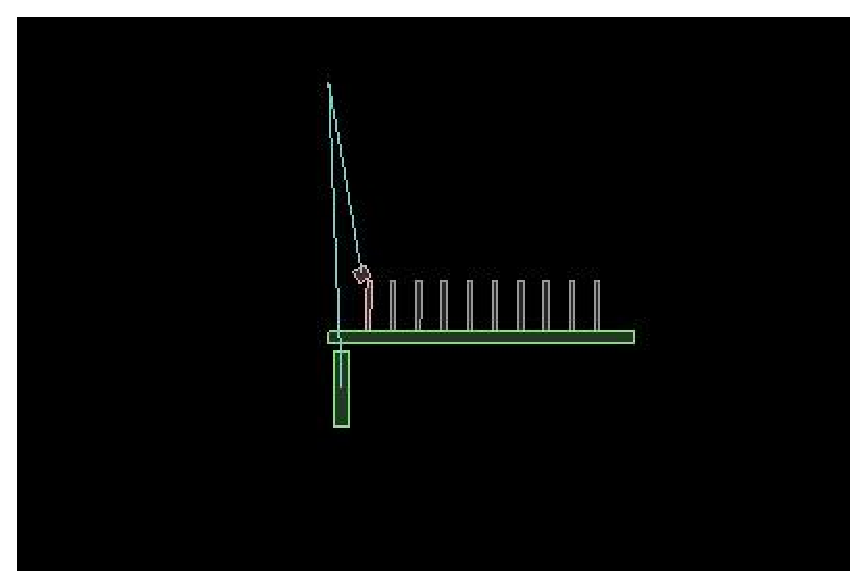
\includegraphics[scale=0.5]{pendulum}
\end{center}
The project simulation consists of 5 pendulums out of which 4 form a Newton's cradle like structure. The bob of the one independent pendulum 
Let the bob of the pendulum\cite{pendulum} be released at an initial angle $\theta_o$  from vertical. Then the speed of the bob, $v$ at an angle $\theta$  will be given by the formula :
\begin{equation}
                                                  v = \sqrt{\frac{2gl}{m}(\cos\theta - \cos\theta_o)}
\end{equation}
where $v$ is in \emph{meters/second}, $g$ is acceleration due to gravity in \emph{meters/second$^2$}, $l$ is the length of the string of pendulum in \emph{meters}, $m$ is the mass of bob in \emph{kilograms}, $\theta$ and $\theta_o$ are in \emph{radian}.

\subsection{Pulley System}
\begin{center}
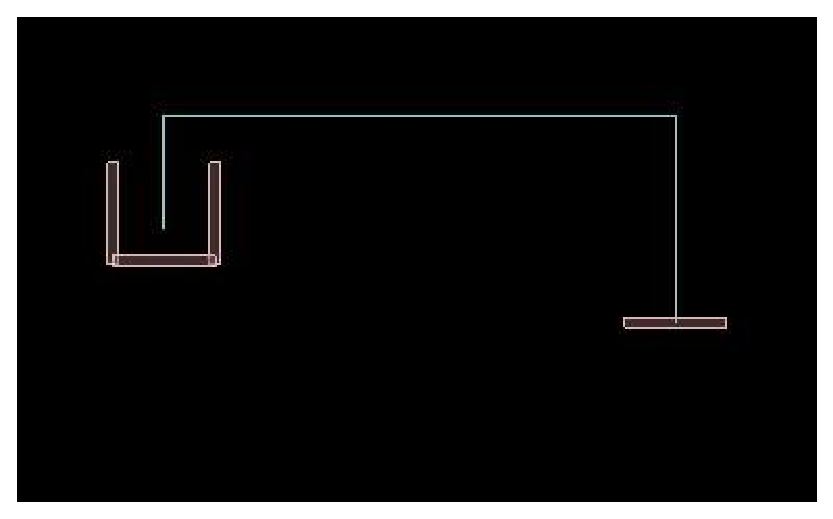
\includegraphics[scale=0.5]{pulley}
\end{center}
This pulley\cite{pulley} system contains weights on both sides. Let the masses be $m_1$ and $m_2$. Then the acceleration $a$ of the weights will be :
\begin{equation}
                                                   a = \frac{m_1 - m_2}{m_1 + m_2}g \mbox{ (assuming $m_1 \geq m_2$)}
\end{equation}
where $a$ is in \emph{meters/second$^2$}, $m_1$ and $m_2$ are in \emph{kilograms} and $g$ is acceleration due to gravity in \emph{meters/second$^2$}.\\*\\*
When the weights have travelled a distance of height $h$, then the speed of the weights, $v$ will be given by the following equation :
\begin{equation}
                                                 v = \sqrt{\frac{2a}{h}} \mbox{ (where $a$ is as used in (2))}
\end{equation}
where $v$ is in \emph{meters/second} and $h$ is in \emph{meters}.

\subsection{Mass Cubical Blocks}
\begin{center}
\includegraphics[scale=0.5]{Mass Cubical Blocks}
\end{center}
When torque\cite{seesaw} is applied to a rod which is hinged at the centre, then the object of mass $m$ kept at some distance $l$ from the hinge experience force. Thus the equation governig this system is as follows :
\begin{equation}
  \vec{\tau} = \frac{ml^2}{12} \times \vec{\alpha}
\end{equation}
where $\vec{\tau}$ is a vector whose magnitude is the torque applied and is measured in \emph{Newton.meter}, $m$ is in \emph{kilograms}, $l$ is in \emph{meters}, $\vec{\alpha}$ is the angular acceleration vector of the object and its magnitude is measured in \emph{radian/second$^2$}.
\section{Conclusions}
We mentioned three systems in the report, namely pendulum, pulley and see-saw, and explained their functioning using mathematical equations which they follow.
\bibliographystyle{plain}
\bibliography{mybib}
\end{document}
